%% ==============================================
%%               Use Cases
%% ==============================================
%% Author: Fabian Sorn
%% ==============================================

\chapter{Use Cases}
\label{ch:usecases}

This chapter will give an overview over different scenarios that we will use for
the evaluation of the Plotting Libraries. All of these originate from teams at
CERN, that are looking into PyQt as an option to implement different \gls{gui}
applications, which also contain plots in them.


%% ==============================================
%%               BE-CO-HT
%% ==============================================
\section{Distributed Oscilloscope for BE-CO-HT}
\label{sec:usecases:becoht}

The first project interested in visualizing data using python graph libraries is
the Distributed Oscilloscope developed in the \gls{ht} section, who are
responsible for the development, production and support for the custom
electronic modules used in the Control System. The goal of the Digital
Oscilloscope is to synchronously monitor analog signals in a distributed system.
To achieve this synchronization, the signals from various sources are
time-stamped and sent to the \gls{gui}, where they can be displayed using
graphs. The project is distributed into three architectural layers, which are
depicted in figure \ref{fig:doarchitecture}.

\begin{figure}[h]
    \centering
    
\includegraphics[width=8cm]{resources/img/DoArchitecture}
    \caption{Digital Oscilloscope Architecture}
    \label{fig:doarchitecture}
\end{figure}

The layer closest to the hardware the depicted signals originate from, are the
device applications, which provide access to hardware resources. The central
layer is the Digital Oscilloscope Server, which is responsible for managing all
connections between device and user applications. The last layer closest to the
users are the user applications. The application our use case originates from,
is a \gls{gui} application representing a oscilloscope, a device for displaying
varying signal voltages over time. A screenshot of this application can be seen
in figure \ref{fig:dogui}.
\cite{DistrOscDocs, BeCoHtSection}

\begin{figure}[h]
    \centering
    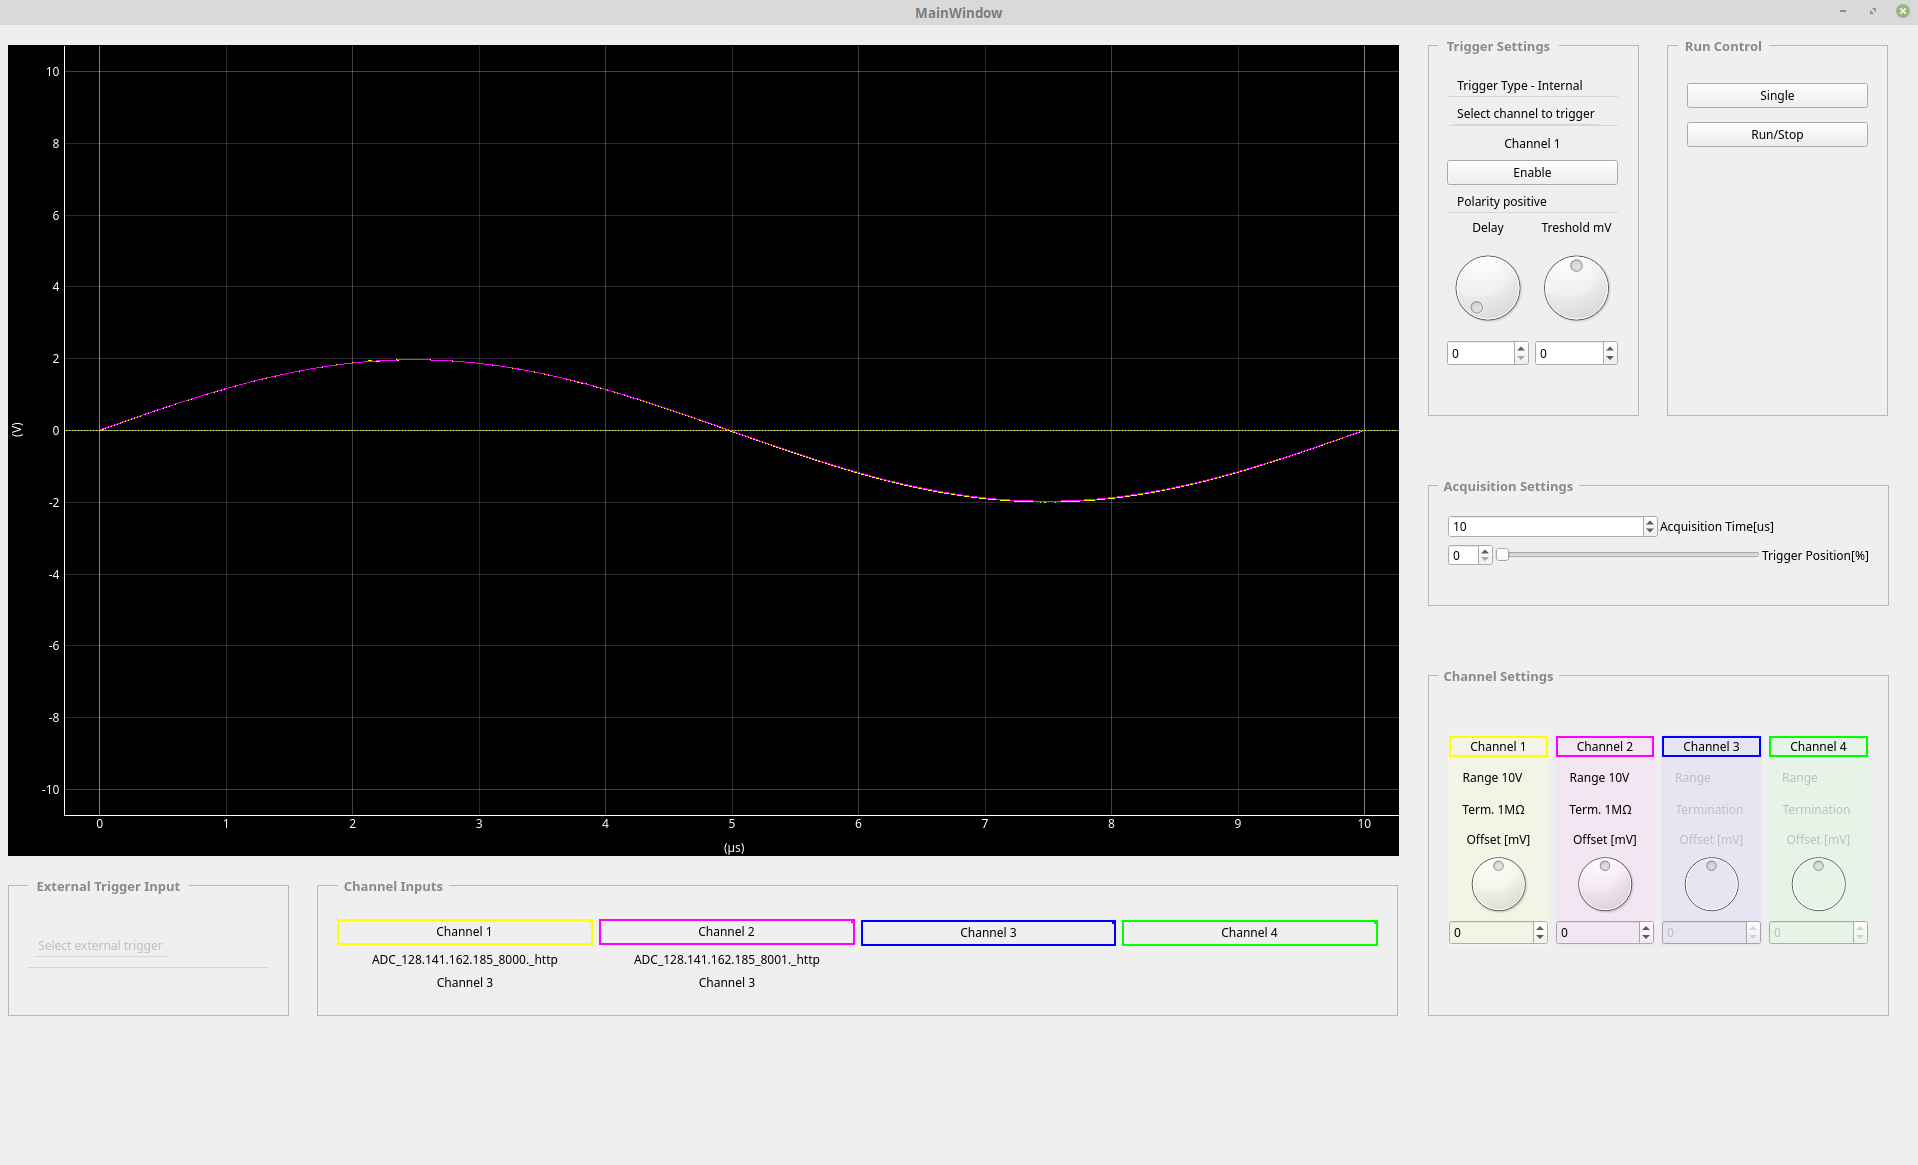
\includegraphics[width=15cm]{resources/img/DistributedOscilloscope}
    \caption{
        Distributed Oscilloscope GUI application displaying two analog signals
    }
    \label{fig:dogui}
\end{figure}

For this \gls{gui}, \gls{ht} is interested in displaying a plot in their
application, which is showing up to eight curves with up to 100.000 points per
curve. The goal for this graph would be an update rate of 25 updates per second.


%% ==============================================
%%               BE-OP-LHC
%% ==============================================
\section{Line Charts in section BE-OP-LHC}
\label{sec:usecases:becolhc}

The second Use Case we will investigate is coming from the \gls{lhcop}, who are
interested in displaying a Line Graph containing 3000 datasets displayed as
curves, who each will contain 2 * 3600 points. The data will be updated every
second.


%% ==============================================
%%               BE-CO-APS
%% ==============================================
\section{Linac4 Source GUI for BE-CO-APS}
\label{sec:usecases:linac}

The third use case originates from \gls{aps}. For this, multiple scatter plots
should be displayed. The \gls{gui} Application will contain 4 different scatter
plots, each containing up to 3 data sets, which each contain 1 hour of live
data, which receives a new point roughly every 1.2 seconds. This results in 3000
visible points per data set.

\begin{figure}[h]
    \centering
    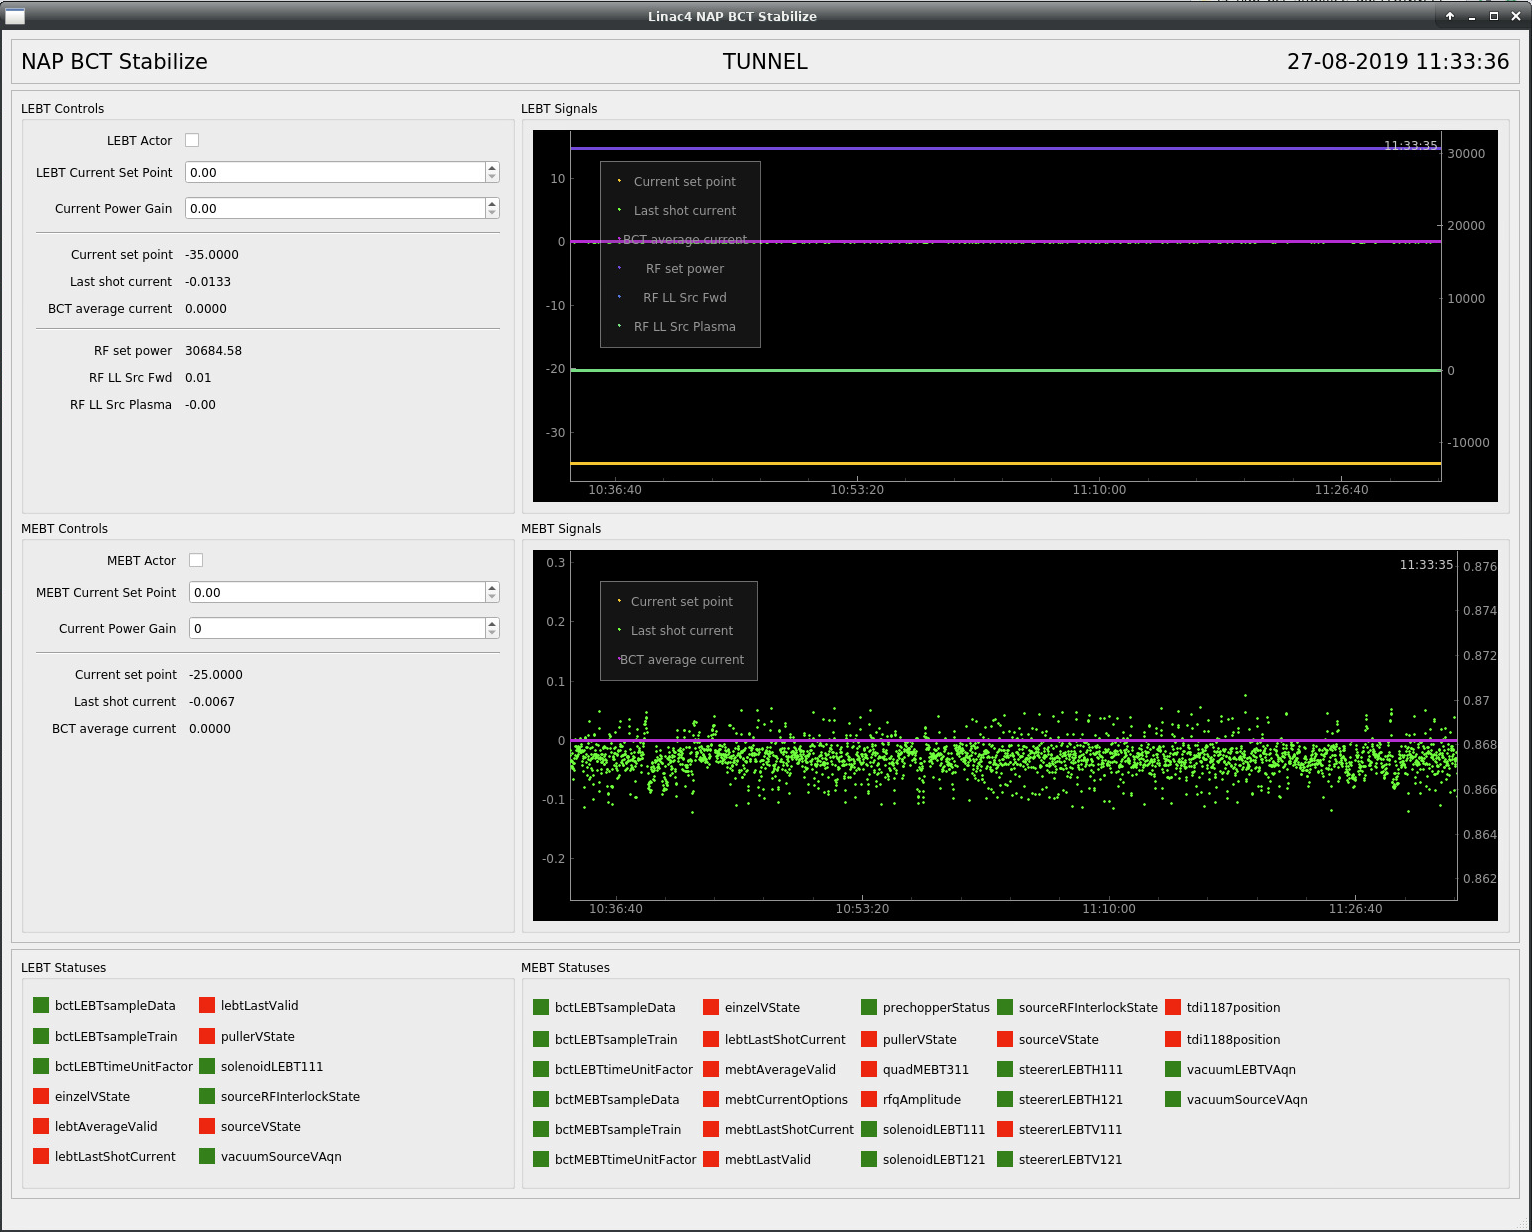
\includegraphics[width=15cm]{resources/img/Linac4SourceGui}
    \caption{Screenshot of the Linac4 Source Gui}
    \label{fig:linac4sourcegui}
\end{figure}

The Application where this Use Case is originated from is a \gls{gui} for the
Linear Accelerator Linac4, whose tasks it is to boost negative hydrogen ions to
high energies. The GUI will allow monitoring and manipulation of different
device settings. Image \ref{fig:linac4sourcegui} shows a screenshot of an early
version of the application with multiple scatter plots in the upper right part
of the window.
\cite{LinacFour,LinacFourGuiPres}

%% ==============================================
%%       Performance Metrics from Use Cases
%% ==============================================
\section{Performance Metrics for User Interfaces}
\label{sec:usecases:metrics}

All of these Use Cases have in common, that they are displaying live data, which
will be delivered with a certain frequency. This means that the graph has only a
certain time to redraw until the next bunch of data arrives. Even for
applications containing graphs, which are not updated regularly, the time it
takes the graph to redraw is very important for the user interaction. Slow
redraw times will lead to stuttering user interfaces. As a result our highest
priority when investigating the performance of plotting libraries should be the
redraw speed of the graph.

From a Usability Engineering perspective, rendering performance is a vital
aspect, since it greatly impacts \glspl{gui} response times. The general
boundary, in which a systems feels like it is responding instantly to a users
interaction is 100 milliseconds. Delays over one second can already interrupt
the thought process of the user, since the delay is getting very noticeable.
Delays over ten seconds require feedback from the system to
signal the user it is performing long running tasks.
\cite{UsabilityEngineering}

An often used measurements for describing a system's rendering performance is the
frame rate, which describes the frequency, with which images appear on a screen.
This size originates from the movie industry, where the standard frame rate is 24
Frames per Second. The minimum frequency needed for the human eye to see a
consecutive movement from a sequence of images is as low as 16 Frames per
Second. This does not mean, that frame rates beyond this won't be recognized by
the human eye. Increasing the Frame Rate leads to the reduction of motion blur,
increasing details and clarity of a moving image.

Especially in the area of computer games, high frame rates are desirable, since
they will not only enhance the visual experience, but give the player a
strategic advantage in a competitive environment.  A popular demonstration of
the increased clarity of high frame rates is the Blur Buster's UFO Motion Blur
Test website, which shows the same scene of fast moving cartoon UFO in different
frame rates (https://www.testufo.com).

In many Hardware Benchmarks, frame rates can be found as the central description
of a hardware component's abilities to render a complex scene. To measure this,
the hardware benchmark will try to rerender the scene as fast as possible. At
the same step in the rendering process of a single frame or image, the current
time stamp is recorded. From these series of timestamps we can calculate the
difference between two adjacent timestamps. This concept is known as Delta
Timing and gives us information, how long the rendering process is taking us per
Frame. Next to a performance description, delta timing can also have other
usages. In Video Games for example, it allows us to find out, how far an object
in the displayed scene should have moved since the last displayed frame. As a
result, figure movement stays consistent, even with different frame rates under
different load scenarios.
\cite{DeltaTiming}

From the recorded timing information, we can calculate the frame rate $f$ from a
set of $m$ recorded time stamps $t_n$ as follows.
\cite{FrameRates}

$$f = \frac{1}{\frac{ \sum_{n=0}^{m-1} t_{n+1} - t_{n} }{ m - 1 }}$$

While frame rates already help us describing performance, they do not yet help
improving it. One way of finding operations in software worth optimizing is
profiling it.  Profilers are software tools which are able to measure different
aspects of performance, like execution time, memory management, garbage
collection and more. The type of profiler we will focus on is deterministic CPU
utilization profilers, which give us information about the time spent in
functions, the callers of it and the number of calls to them. Next to finding
slow performing functions, they can uncover as well, if a function is called
more often as intended by a programs author. With this information, optimization
efforts can be directed to where they really can make a difference.
\cite{CProfilerExample}

The standard option in Python for deterministic profiling, is the C extension
\emph{cProfile}. Compared to the profiler \emph{profile}, which itself is
written in Python, cProfile offers a much lower overhead, which makes it
suitable for profiling longer running programs.  To provide collect information
about the execution of a program, cProfile uses hooks for events, which are
offered by the Python interpreter. These hooks are callbacks, which allow
cProfile to receive and record timing information about every function executed.
For profile and cProfile, there are two limitations, which you have to be aware
of. The first one is the granularity of the underlying
timer used for recording the duration of an operation. On most systems this is
around 0.001 seconds.  The other limitation is the lag between the event being
dispatched and the profiler getting the current time. Since profiling is
introducing a certain overhead to the execution of a python program, it is not
suitable for benchmarking itself.
\cite{CProfiler}
